%%
%% Beginning of file 'sample61.tex'
%%
%% Modified 2016 September
%%
%% This is a sample manuscript marked up using the
%% AASTeX v6.1 LaTeX 2e macros.
%%
%% AASTeX is now based on Alexey Vikhlinin's emulateapj.cls 
%% (Copyright 2000-2015).  See the classfile for details.

%% AASTeX requires revtex4-1.cls (http://publish.aps.org/revtex4/) and
%% other external packages (latexsym, graphicx, amssymb, longtable, and epsf).
%% All of these external packages should already be present in the modern TeX 
%% distributions.  If not they can also be obtained at www.ctan.org.

%% The first piece of markup in an AASTeX v6.x document is the \documentclass
%% command. LaTeX will ignore any data that comes before this command. The 
%% documentclass can take an optional argument to modify the output style.
%% The command below calls the preprint style  which will produce a tightly 
%% typeset, one-column, single-spaced document.  It is the default and thus
%% does not need to be explicitly stated.
%%
%%
%% using aastex version 6.1
\documentclass[twocolumn]{aastex62}

%% The default is a single spaced, 10 point font, single spaced article.
%% There are 5 other style options available via an optional argument. They
%% can be envoked like this:
%%
%% \documentclass[argument]{aastex61}
%% 
%% where the arguement options are:
%%
%%  twocolumn   : two text columns, 10 point font, single spaced article.
%%                This is the most compact and represent the final published
%%                derived PDF copy of the accepted manuscript from the publisher
%%  manuscript  : one text column, 12 point font, double spaced article.
%%  preprint    : one text column, 12 point font, single spaced article.  
%%  preprint2   : two text columns, 12 point font, single spaced article.
%%  modern      : a stylish, single text column, 12 point font, article with
%% 		  wider left and right margins. This uses the Daniel
%% 		  Foreman-Mackey and David Hogg design.
%%
%% Note that you can submit to the AAS Journals in any of these 6 styles.
%%
%% There are other optional arguments one can envoke to allow other stylistic
%% actions. The available options are:
%%
%%  astrosymb    : Loads Astrosymb font and define \astrocommands. 
%%  tighten      : Makes baselineskip slightly smaller, only works with 
%%                 the twocolumn substyle.
%%  times        : uses times font instead of the default
%%  linenumbers  : turn on lineno package.
%%  trackchanges : required to see the revision mark up and print its output
%%  longauthor   : Do not use the more compressed footnote style (default) for 
%%                 the author/collaboration/affiliations. Instead print all
%%                 affiliation information after each name. Creates a much
%%                 long author list but may be desirable for short author papers
%%
%% these can be used in any combination, e.g.
%%
%% \documentclass[twocolumn,linenumbers,trackchanges]{aastex61}

%% AASTeX v6.* now includes \hyperref support. While we have built in specific
%% defaults into the classfile you can manually override them with the
%% \hypersetup command. For example,
%%
%%\hypersetup{linkcolor=red,citecolor=green,filecolor=cyan,urlcolor=magenta}
%%
%% will change the color of the internal links to red, the links to the
%% bibliography to green, the file links to cyan, and the external links to
%% magenta. Additional information on \hyperref options can be found here:
%% https://www.tug.org/applications/hyperref/manual.html#x1-40003

%% If you want to create your own macros, you can do so
%% using \newcommand. Your macros should appear before
%% the \begin{document} command.
%%
\usepackage{multirow}
\newcommand{\vdag}{(v)^\dagger}
\newcommand\aastex{AAS\TeX}
\newcommand\latex{La\TeX}
\newcommand{\sm}{M_\odot}
\newcommand{\sr}{R_\odot}

%% Reintroduced the \received and \accepted commands from AASTeX v5.2
\received{\today}
\revised{}
\accepted{}
%% Command to document which AAS Journal the manuscript was submitted to.
%% Adds "Submitted to " the arguement.
\submitjournal{PASP}

%% Mark up commands to limit the number of authors on the front page.
%% Note that in AASTeX v6.1 a \collaboration call (see below) counts as
%% an author in this case.
%
%\AuthorCollaborationLimit=3
%
%% Will only show Schwarz, Muench and "the AAS Journals Data Scientist 
%% collaboration" on the front page of this example manuscript.
%%
%% Note that all of the author will be shown in the published article.
%% This feature is meant to be used prior to acceptance to make the
%% front end of a long author article more manageable. Please do not use
%% this functionality for manuscripts with less than 20 authors. Conversely,
%% please do use this when the number of authors exceeds 40.
%%
%% Use \allauthors at the manuscript end to show the full author list.
%% This command should only be used with \AuthorCollaborationLimit is used.

%% The following command can be used to set the latex table counters.  It
%% is needed in this document because it uses a mix of latex tabular and
%% AASTeX deluxetables.  In general it should not be needed.
%\setcounter{table}{1}

%%%%%%%%%%%%%%%%%%%%%%%%%%%%%%%%%%%%%%%%%%%%%%%%%%%%%%%%%%%%%%%%%%%%%%%%%%%%%%%%
%%
%% The following section outlines numerous optional output that
%% can be displayed in the front matter or as running meta-data.
%%
%% If you wish, you may supply running head information, although
%% this information may be modified by the editorial offices.
\shorttitle{PS1 Star-galaxy Catalog}
\shortauthors{One then the other}
%%
%% You can add a light gray and diagonal water-mark to the first page 
%% with this command:
\watermark{DRAFT}
%% where "text", e.g. DRAFT, is the text to appear.  If the text is 
%% long you can control the water-mark size with:
%  \setwatermarkfontsize{dimension}
%% where dimension is any recognized LaTeX dimension, e.g. pt, in, etc.
%%
%%%%%%%%%%%%%%%%%%%%%%%%%%%%%%%%%%%%%%%%%%%%%%%%%%%%%%%%%%%%%%%%%%%%%%%%%%%%%%%%

%%%%%%%%%%%%%%%%%%%%%%%%%%%%%%%%%%%%%%%%%%%%%%%%%%%%%%%%%%%%%%%%%%%%%%%%%%%%%%%%
%%
%% The following section defines new commands for comments from co-authors
%%
\newcommand{\yutaro}[1]{{\color{red} yt: {#1}}}
\newcommand{\aam}[1]{{\color{blue} aam: {#1}}}
\newcommand{\todo}[1]{{\color{magenta} to-do: {#1}}}
%%
%%%%%%%%%%%%%%%%%%%%%%%%%%%%%%%%%%%%%%%%%%%%%%%%%%%%%%%%%%%%%%%%%%%%%%%%%%%%%%%%

%% This is the end of the preamble.  Indicate the beginning of the
%% manuscript itself with \begin{document}.

\begin{document}

\title{\textbf{something better needed} A Machine Learning Model to Separate Stars and Galaxies in PanSTARRS1 Data}

%% LaTeX will automatically break titles if they run longer than
%% one line. However, you may use \\ to force a line break if
%% you desire. In v6.1 you can include a footnote in the title.

%% A significant change from earlier AASTEX versions is in the structure for 
%% calling author and affilations. The change was necessary to implement 
%% autoindexing of affilations which prior was a manual process that could 
%% easily be tedious in large author manuscripts.
%%
%% The \author command is the same as before except it now takes an optional
%% arguement which is the 16 digit ORCID. The syntax is:
%% \author[xxxx-xxxx-xxxx-xxxx]{Author Name}
%%
%% This will hyperlink the author name to the author's ORCID page. Note that
%% during compilation, LaTeX will do some limited checking of the format of
%% the ID to make sure it is valid.
%%
%% Use \affiliation for affiliation information. The old \affil is now aliased
%% to \affiliation. AASTeX v6.1 will automatically index these in the header.
%% When a duplicate is found its index will be the same as its previous entry.
%%
%% Note that \altaffilmark and \altaffiltext have been removed and thus 
%% can not be used to document secondary affiliations. If they are used latex
%% will issue a specific error message and quit. Please use multiple 
%% \affiliation calls for to document more than one affiliation.
%%
%% The new \altaffiliation can be used to indicate some secondary information
%% such as fellowships. This command produces a non-numeric footnote that is
%% set away from the numeric \affiliation footnotes.  NOTE that if an
%% \altaffiliation command is used it must come BEFORE the \affiliation call,
%% right after the \author command, in order to place the footnotes in
%% the proper location.
%%
%% Use \email to set provide email addresses. Each \email will appear on its
%% own line so you can put multiple email address in one \email call. A new
%% \correspondingauthor command is available in V6.1 to identify the
%% corresponding author of the manuscript. It is the author's responsibility
%% to make sure this name is also in the author list.
%%
%% While authors can be grouped inside the same \author and \affiliation
%% commands it is better to have a single author for each. This allows for
%% one to exploit all the new benefits and should make book-keeping easier.
%%
%% If done correctly the peer review system will be able to
%% automatically put the author and affiliation information from the manuscript
%% and save the corresponding author the trouble of entering it by hand.

\correspondingauthor{A.~A.~Miller}
\email{amiller@northestern.edu}

% \author[0000-0001-9515-478X]{A.~A.~Miller}
% \affil{Center for Interdisciplinary Exploration and Research in Astrophysics (CIERA) and Department of Physics and Astronomy, Northwestern University, 2145 Sheridan Road, Evanston, IL 60208, USA}
% \affil{The Adler Planetarium, Chicago, IL 60605, USA}

\author{Concerned ZTF Scientists}
\affil{Zwicky Transient Facility}

%% Note that the \and command from previous versions of AASTeX is now
%% depreciated in this version as it is no longer necessary. AASTeX 
%% automatically takes care of all commas and "and"s between authors names.

%% AASTeX 6.1 has the new \collaboration and \nocollaboration commands to
%% provide the collaboration status of a group of authors. These commands 
%% can be used either before or after the list of corresponding authors. The
%% argument for \collaboration is the collaboration identifier. Authors are
%% encouraged to surround collaboration identifiers with ()s. The 
%% \nocollaboration command takes no argument and exists to indicate that
%% the nearby authors are not part of surrounding collaborations.

%% Mark off the abstract in the ``abstract'' environment. 
\begin{abstract}

We did a decent job of separating stars and galaxies.

\end{abstract}

%% Keywords should appear after the \end{abstract} command. 
%% See the online documentation for the full list of available subject
%% keywords and the rules for their use.
\keywords{catalogs --- galaxies: statistics \UTF{2013}-- methods: data analysis \UTF{2013}-- methods: statistical --\UTF{2013} stars: statistics --- surveys}

%% From the front matter, we move on to the body of the paper.
%% Sections are demarcated by \section and \subsection, respectively.
%% Observe the use of the LaTeX \label
%% command after the \subsection to give a symbolic KEY to the
%% subsection for cross-referencing in a \ref command.
%% You can use LaTeX's \ref and \label commands to keep track of
%% cross-references to sections, equations, tables, and figures.
%% That way, if you change the order of any elements, LaTeX will
%% automatically renumber them.

%% We recommend that authors also use the natbib \citep
%% and \citet commands to identify citations.  The citations are
%% tied to the reference list via symbolic KEYs. The KEY corresponds
%% to the KEY in the \bibitem in the reference list below. 

\section{Introduction}
\label{sec:intro}

\yutaro{define ps1}

\section{Model Data}

Data for the star-galaxy model were obtained from the PS1 casjobs server.\footnote{http://mastweb.stsci.edu/ps1casjobs/home.aspx} The PS1 database provides flux measurements via aperture photometry, point-spread-function (PSF) photometry, and \citet{Kron80} photometry.\footnote{A subset of bright sources ($i < 21\,\mathrm{mag}$) outside the Galactic plane have additional photometric measurements, e.g., exponential or \citet{Sersic63} profiles, in the \textit{StackModelFitExp} and \textit{StackModelFitSer} tables, respectively. We ignore these measurements for this study as they are not available for all sources.} These flux measurements are produced by PS1 in 3 different ways. The mean brightness measured on the individual PS1 frames is reported in the \textit{MeanObject} table, the mean brightness measured via forced-PSF/aperture photometry on the individual PS1 frames is reported in the \textit{ForcedMeanObject} table, and finally, the brightness measured on the full-depth stacked PS1 images is reported in the \textit{StackObjectThin} table. The \textit{StackObjectAttributes} table further supplements these tables with point-source object shape measurements, which are very useful to discriminate stars and galaxies. Ultimately, see \S\ref{sec:simple_model}, we use flux measurements from the \textit{StackObjectThin} table and shape measurements from the \textit{StackObjectAttributes} to build our models.

\subsection{The \textit{HST} Training Set} 

A fundamental challenge in the construction of any supervised machine learning model is the curation of a high-fidelity training set. A subset of the data that requires classification must have known labels so that the machine can learn the proper mapping between features and labels. The superior image quality of the \textit{Hubble Space Telescope} (\textit{HST}) provides exceptionally accurate morphological classifications, making it an ideal source of a training set for lower quality ground-based imaging (e.g., \citealt{Lupton01}). The downside of \textit{HST} is that the field of view is relatively small, so it is difficult to construct a large and diverse training set suitable for predictions over the entire sky. 

We use the largest contiguous area imaged by \textit{HST}, the 1.64\,deg$^2$
COSMOS field, to construct a training set for our models. Morphological
classifications of \textit{HST} COSMOS sources are provided in
\citet{Leauthaud07}. \citeauthor{Leauthaud07} demonstrate reliable
classifications down to $\sim$25\,mag, which is significantly deeper than the
faintest sources detected by PS1. We identify counterparts in the PS1 and
\textit{HST} data by performing a spatial crossmatch between the two catalogs
using a 1\arcsec radius.\footnote{This matching radius is the same employed
by PS1 to associate individual detections in the \textit{MeanObject} table
with detections in the \textit{StackObjectAttributes} table.} 
\yutaro{I think
there may be more details here for the filtering of this data - did you
exclude some matches based on \texttt{MAG\_AUTO}, or something similar to
that?
$\leftarrow$ When we used \textit{StackObjectThin}, 
I actually excluded sources with \texttt{MAG\_AUTO} $>$ 25 mag 
because they are likely mis-crossmatched source 
which is too faint to be detected PS1 and is within a 1\arcsec radius 
from another PS1 source. 
However in \textit{MeanObjectThin} the number of such source is very small, 
so I did not perform the filtering for the final model.} 
Following this procedure, we find that there are 87,431 sources in the
\citet{Leauthaud07} catalog with PS1 counterparts. Of these, 80,974 are
unique in that there is a one-to-one correspondence between \textit{HST}
source and a single PS1 \textit{ObjID}. The training set is further reduced
to 75,927 once our detection criteria are applied (see
\S\ref{sec:simple_model}), and, of those, only 47,093 have
$\texttt{nDetections} \ge 1$ in the PS1 database.

\todo{Is there an interesting figure to show here that isn't redundant with other figures that we will show?}

% \begin{figure}[]
%   \centering
%   \includegraphics[width=3.35in]{.pdf}
%   \caption{ }
%   %
%   \label{fig:}
% \end{figure}

\section{Model Construction}
\subsection{The PS1 Baseline Model}\label{sec:ps1_model}

To establish a baseline for the performance of our star-galaxy separation models we adopt the classification criteria in the PS1 documentation, namely sources with
$$ \mathtt{iPSFMag} - \mathtt{iKronMag} > 0.05\;\mathrm{mag},$$
are classified as galaxies.\footnote{\url{https://outerspace.stsci.edu/display/PANSTARRS/How+to+separate+stars+and+galaxies}} The documentation notes that this classification can be performed using photometry from any of the \textit{MeanObject}, \textit{ForcedMeanObject}, or \textit{StackedObjectThin} tables. The PS1 documentation further notes that this basic cut does not perform well for sources with $i \gtrsim 21\,\mathrm{mag}$, which constitutes the majority of sources detected by PS1, and motivates us to generate our own star-galaxy separation models. We use the performance of the $\mathtt{iPSFMag} - \mathtt{iKronMag} > 0.05\;\mathrm{mag}$ model (hereafter, the PS1 model) as a baseline to compare to the models discussed below.

\subsection{Simple Model}\label{sec:simple_model}
\yutaro{
Since only the i-band photometric measurement is used for the star-galaxy separation  
in the PS1 model as explained in \S\ref{sec:simple_model},  
it is expected that the separation accuracy is improved 
by the model with the photometric measurement in all of the five optical bands 
provided by PS1 (g, r, i, z, and y), especially for the source 
detected with a higher signal to noise ratio (S/N) by the other band than that of i-band. 
We therefore created a simple model (hereafter, the simple model) for the separation 
with the photometric measurement in all of the optical bands 
for referring it as a new strict baseline model for the machine learning model  
we developed (described in \S\ref{sec:rf_model}).

The essential idea for the separation by the simple model is the same as the PS1 model;  
sources with a ratio of the $\mathtt{KronFlux}$ to the $\mathtt{PSFFlux}$ 
(corresponding to $\mathtt{PSFMag} - \mathtt{KronMag}$) larger than a threshold 
are classified as galaxies, 
but instead of $\mathtt{i[PSF, Kron]Mag}$,  
we use the white flux measurements ($\mathtt{w[PSF,Kron]Flux}$) 
defined by the weighted average of the flux in all of the optical band:   
$$
\mathtt{w[PSF, Kron]Flux} =  \frac{\sum w_c  F_c }{\sum w_c}, 
\ w_c = \left( \frac{F_c}{e_c} \right)^2, 
$$
where $c = [\mathtt{g, r, i, z, y}]$,  $F$ is the $\mathtt{[PSF,Kron]Flux}$, 
and $e$ is the $\mathtt{[PSF,Kron]FluxErr}$.  
The weight $w = \mathrm{(S/N)}^2$ allows this model to perform better decision 
than the normal average ($w = 1$) by retaining the flux information with high S/N more stronger. 

In order to evaluate the probability of that each source is a star or a galaxy quantitatively, 
we decided to use the orthogonal distance from the threshold line 
($\mathtt{wPSFFlux} = a\times \mathtt{wKronFlux}$) 
on the $\mathtt{wPSFFlux}$-$\mathtt{wKronFlux}$ plane for the simple model:  
$$
\mathtt{wPSFKronDist}(a) = 
	\frac{\mathtt{wPSFFlux} - a\times\mathtt{wKronFlux}}{ \sqrt{1 + a^2}}, 
$$
where $a$ is the critical ratio of the $\mathtt{wPSFFlux}$ to the $\mathtt{wKronFlux}$ 
(corresponding to 0.05 in the PS1 model). 
A bright source, which can be classified clearly, 
has larger $|\mathtt{wPSFKronDist}|$ than that of a faint source, 
even if the ratio of the $\mathtt{wPSFFlux}$ to the $\mathtt{wKronFlux} $
($\propto \mathtt{wPSFMag}  -  \mathtt{wKronMag}$) of them is the same. 
We therefore can use the $\mathtt{wPSFKronDist}$ directly 
as the likelihood of that the source is a star or a galaxy, 
and furthermore, this treatment improves the true positive ratio (TPR) 
at the low false positive ratio (FPR) dramatically (see \S*** and Fig.\ref{fig:cvroc_hst}). 

In this paper, we use $a=0.91375$ derived by the average of $a$ 
through 10-fold cross variation (CV) procedure;   
the data set is split into 10 smaller sets 
and obtain a $a$ by maximizing the TPR at FPR$ = 0.005$ 
(called figure of merit; FoM) of 9 of the folds. 
We repeat this procedure 10 times in total for all of the combination of 9 of the folds. 
The distribution of the $\mathtt{wPSFKronDist}$ on $a=0.91375$ is shown in Fig.\ref{fig:psfkrondist}. 

\begin{figure}[t]
 \centering
  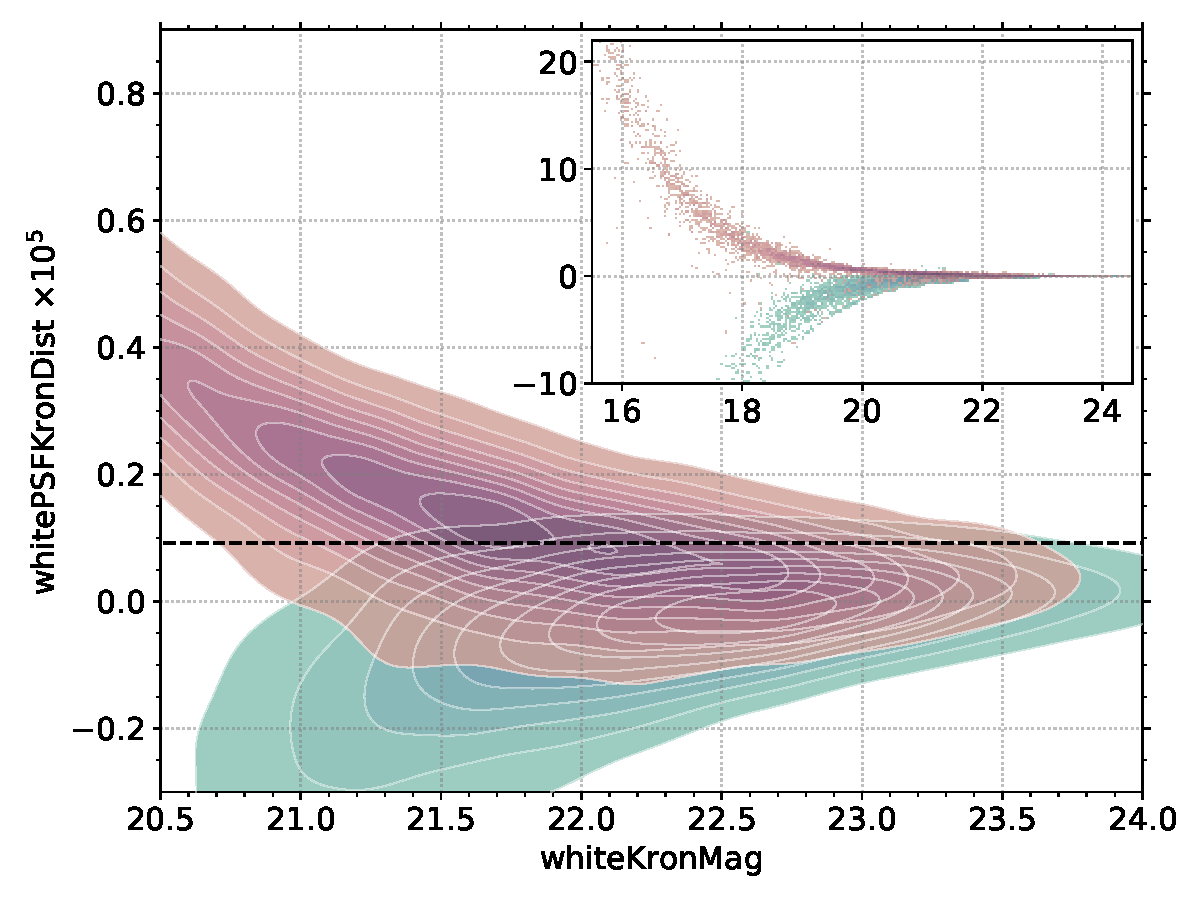
\includegraphics[width=3.35in]{./Figures/whitePSFKronDist.pdf}
%  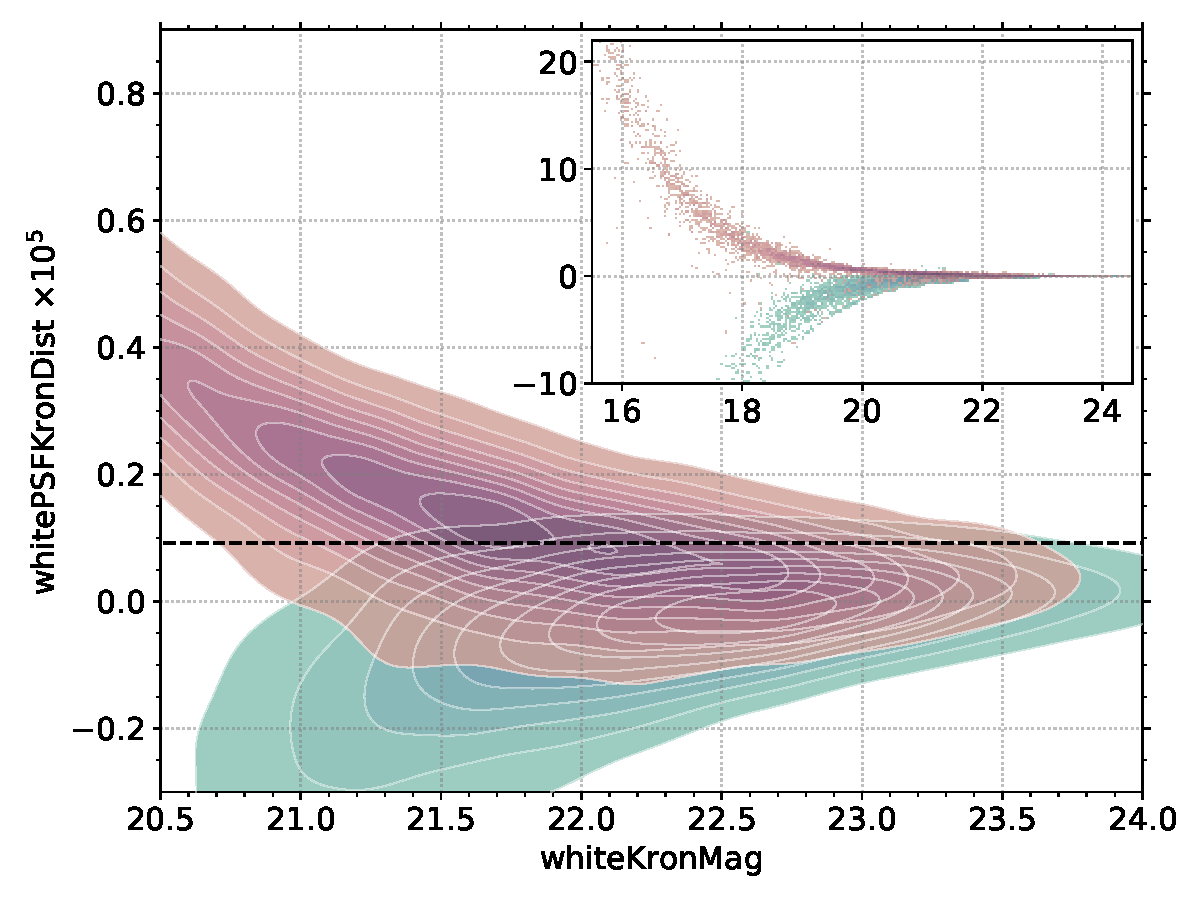
\includegraphics[width=3.35in]{./Figures/whitePSFKronDist.eps}
  \caption{The distribution of the $\mathtt{wPSFKronDist}$. 
We show the entire behavior of the $\mathtt{wPSFKronDist}$ for the stars and galaxies 
in the small window and the KDE of them at the faintest region is shown in the main panel. 
The dashed line represents the threshold maximizing the separation accuracy for HST sources. }
  %
  \label{fig:psfkrondist}
\end{figure}
}


\subsection{Random Forest Model}\label{sec:rf_model}
The random forest model


%%%%%%%%
\begin{table*}
\begin{center}
\caption{The true positive ratio and the threshold 
corresponding to the false positive ratio = 0.005, 0.01, 0.02, 0.05, and 0.1. }
\label{tbl:fpr}
\begin{tabular}{llccccc}
\hline\hline
                                                 & False positive ratio & 0.005 & 0.01 & 0.02 & 0.05 & 0.1 \\ \hline
\multicolumn{1}{l}{\multirow{2}{*}{All sources}} & True positive ratio  & $0.697 \pm 0.008$ &  $0.742 \pm 0.005$ & $0.786 \pm 0.003$ & $0.852 \pm 0.003$ & $0.899 \pm 0.003$  \\
\multicolumn{1}{l}{}                             & Threshold & $0.76 \pm 0.05$ &  $0.65 \pm 0.04$ & $0.53 \pm 0.02$ & $0.36 \pm 0.01$ & $0.24 \pm 0.01$  \\ \hline
\multirow{2}{*}{$\mathtt{rKornMag} < 21$} & True positive ratio  & $0.861 \pm 0.062$ &  $0.953 \pm 0.024$ & $0.986 \pm 0.002$ & $0.993 \pm 0.001$ & $0.996 \pm 0.001$ \\
                                                 & Threshold & $0.82 \pm 0.17$ &  $0.70 \pm 0.18$ & $0.40 \pm 0.10$ & $0.16 \pm 0.06$ & $0.07 \pm 0.03$   \\ \hline
\multirow{2}{*}{$\mathtt{rKornMag} < 20$}  & True positive ratio  & $0.841 \pm 0.075$ &  $0.958 \pm 0.028$ & $0.997 \pm 0.001$ & $0.998 \pm 0.001$ & $0.999 \pm 0.001$  \\
                                                  & Threshold & $0.90 \pm 0.18$ &  $0.81 \pm 0.24$ & $0.77 \pm 0.26$ & $0.13 \pm 0.08$ & $0.06 \pm 0.04$ \\ \hline
\end{tabular}
\end{center}
\end{table*}
%%%%%%%%

\section{Results}

\begin{figure}[t]
 \centering
  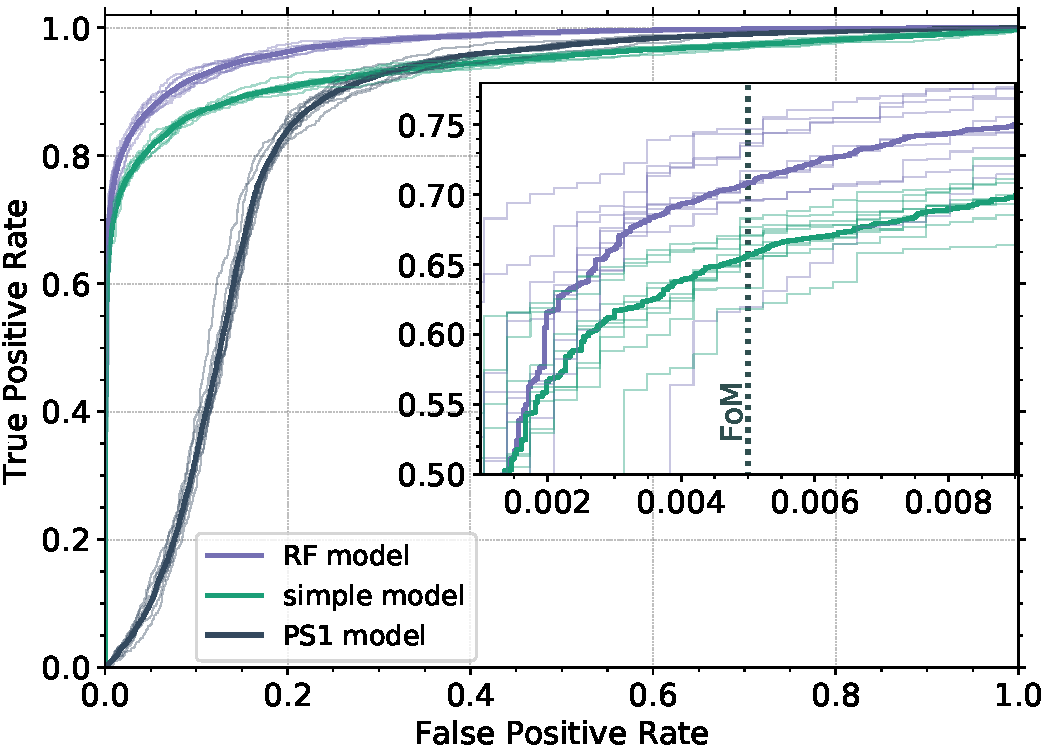
\includegraphics[width=3.35in]{./Figures/CV_ROC_HST.pdf}
%  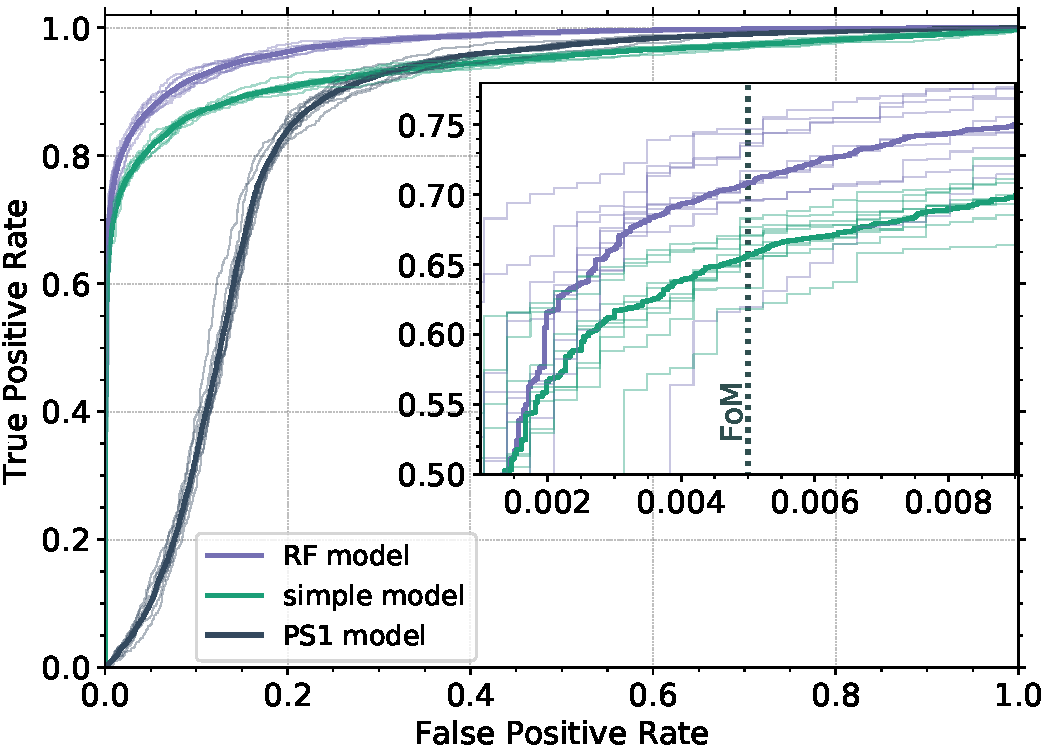
\includegraphics[width=3.35in]{./Figures/CV_ROC_HST.eps}
  \caption{}
  %
  \label{fig:cvroc_hst}
\end{figure}


\section{Discussion}

\section{Conclusions}

\acknowledgements

\begin{itemize}
    \item Brian Bue (possibly also Umaa, check emails)
    \item PS1 casjobs (Bernie in particular)
\end{itemize}

AAM is funded by the Large Synoptic Survey Telescope Corporation in support of
the Data Science Fellowship Program.

\facility{PS1}

\software{\texttt{astropy} \citep{Astropy-Collaboration13},  }.


\appendix


\bibliographystyle{aasjournal}
\bibliography{star_gal}

\end{document}
